\FloatBarrier
\setlength{\intextsep}{6pt}
\section{Experiments}
\label{sec:experiments}
\subsection{Experimental setup}
JAM combines robot demonstrations with human video in embodied pretraining. The current mixture
uses DROID \citep{droid}, BridgeData V2 \citep{bridge}, EgoDex \citep{egodex}, Ego4D \citep{ego4d}, and the
Franka, UR5e, and AgileX portions of RoboMIND \citep{robomind}. Appendix~\ref{app:setup} gives
source counts and sampling probabilities. The 6.02-billion-parameter model combines public video
initialization with a newly initialized agent stream, trained on eight H200 accelerators with
global batch 512. Episode-level holdouts separate training windows from open-loop checks;
benchmark adaptation uses designated training splits, with LIBERO-Plus and LIBERO-PRO reserved
for evaluation.

The evidence snapshot contains foundation optimization through update \FoundationSteps{}, a
completed 20,000-update LIBERO adaptation, and frozen-world diagnostics at update 5,100.
The benchmark tables retain source-reported baseline values and reserve blue rows for JAM
evaluation. Paired comparisons fix demonstrations, adaptation budgets, and environment resets.
Success measures closed-loop control; frozen-feature readouts and input sensitivity assess
representation content. Controlled pretraining and scaling displays retain target markers
while measurements are pending. Appendix~\ref{app:controls} specifies probe sampling and uncertainty.

\subsection{Benchmark control and generalization}
Table~\ref{tab:libero_plus} resolves robustness across seven perturbation axes.
\begin{table}[H]
\centering
\begingroup\fontsize{9.2}{10.5}\selectfont
\setlength{\tabcolsep}{2.5pt}\renewcommand{\arraystretch}{1.08}
\begin{tabularx}{\linewidth}{@{}p{1.43in}CCCCCCCC@{}}
\toprule
\panelrow{9}{LIBERO-Plus}
Model & Camera & Robot & Language & Light & Backgr. & Noise & Layout & Mean \\
\midrule
$\pi_0$ & 13.8 & 6.0 & 58.8 & 85.0 & 81.4 & 79.0 & 68.9 & 53.6 \\
OpenVLA-OFT & 56.4 & 31.9 & 79.5 & 88.7 & 93.3 & 75.8 & 74.2 & 69.6 \\
StarVLA & 52.5 & 49.8 & 88.5 & 95.7 & 95.7 & 73.0 & 76.9 & 74.1 \\
ABot-M0 & 60.4 & 67.9 & 86.4 & 96.2 & 91.6 & 86.4 & 82.6 & 80.5 \\
$\pi_{0.5}$ & 78.4 & 73.6 & 80.8 & 96.2 & 94.1 & 89.0 & 84.5 & 84.4 \\
ACoT-VLA & 72.6 & 82.6 & 87.5 & 97.7 & 96.5 & 87.8 & 88.1 & 86.6 \\
Qwen-RobotManip & \textbf{87.2} & 75.5 & 85.6 & 96.6 & \textbf{97.7} & \textbf{97.7} & 87.3 & \textbf{89.0} \\
\midrule
Fast-WAM & 16.4 & 44.5 & 68.9 & 78.2 & 53.7 & 37.7 & 60.7 & 51.5 \\
Being-H0.7 & 82.0 & 59.0 & 82.8 & 97.8 & 90.0 & 93.5 & \textbf{88.5} & 82.1 \\
Cosmos Policy & 75.8 & 63.3 & 81.7 & 96.5 & 88.9 & 92.7 & 82.2 & 82.2 \\
ImageWAM & 80.8 & 50.3 & \textbf{91.4} & \textbf{98.1} & 85.5 & 93.8 & 80.5 & 83.1 \\
ABot-M0.5 & 70.5 & \textbf{87.4} & 88.6 & 94.0 & 89.7 & 75.5 & 85.2 & 83.4 \\
R1 & 33.8 & 76.1 & 88.0 & 97.0 & 87.1 & 39.8 & 77.5 & 69.2 \\
\midrule
\jamshade\textbf{JAM} & \multicolumn{8}{c}{\pendingresult} \\
\bottomrule
\end{tabularx}
\endgroup
\caption{\textbf{LIBERO-Plus robustness.} Success percentages across all seven perturbation axes; the reported mean retains the source aggregation. Source: \refsource{}. \benchmarknote}
\label{tab:libero_plus}
\end{table}

\FloatBarrier
Table~\ref{tab:libero_pro} summarizes robustness within four task suites.
\begin{table}[H]
\centering
\begingroup\fontsize{8.7}{10.0}\selectfont
\setlength{\tabcolsep}{2.5pt}\renewcommand{\arraystretch}{1.08}
\begin{tabularx}{\linewidth}{@{}p{.92in}CCCCCCCCCC@{}}
\toprule
\panelrow{11}{A. Goal and spatial control}
Model & \multicolumn{5}{c}{Goal} & \multicolumn{5}{c}{Spatial} \\
\cmidrule(lr){2-6}\cmidrule(lr){7-11}
 & Obj. & Pos. & Sem. & Task & Env. & Obj. & Pos. & Sem. & Task & Env. \\
\midrule
OpenVLA & 96 & 0 & 98 & 0 & 98 & 97 & 0 & 97 & 0 & 89 \\
$\pi_0$ & 94 & 0 & 93 & 0 & 39 & 95 & 0 & 97 & 0 & 60 \\
$\pi_{0.5}$ & 97 & 38 & 97 & 0 & 46 & 97 & 20 & 97 & 1 & 46 \\
MolmoAct & 68 & 0 & 85 & 0 & \nr & 90 & 0 & 88 & 0 & \nr \\
NORA & 58 & 0 & 88 & 0 & \nr & 92 & 0 & 91 & 0 & \nr \\
X-VLA & 68 & 1 & 98 & 9 & \nr & 97 & 0 & 96 & 0 & \nr \\
\bottomrule
\end{tabularx}
\vspace{3pt}
\begin{tabularx}{\linewidth}{@{}p{.92in}CCCCCCCCCCC@{}}
\toprule
\panelrow{12}{B. Long-horizon and object control}
Model & \multicolumn{5}{c}{Long} & \multicolumn{5}{c}{Object} & Total \\
\cmidrule(lr){2-6}\cmidrule(lr){7-11}
 & Obj. & Pos. & Sem. & Task & Env. & Obj. & Pos. & Sem. & Task & Env. & Rep. \\
\midrule
OpenVLA & 81 & 0 & 96 & 0 & 85 & 98 & 0 & 98 & 0 & 0 & 52 \\
$\pi_0$ & 79 & 0 & 82 & 0 & 27 & 94 & 0 & 90 & 0 & 29 & 44 \\
$\pi_{0.5}$ & 92 & 8 & 93 & 1 & 46 & 98 & 17 & 96 & 1 & 73 & 53 \\
MolmoAct & 54 & 0 & 74 & 6 & \nr & 92 & 6 & 96 & 0 & \nr & 41 \\
NORA & 46 & 0 & 74 & 0 & \nr & 86 & 0 & 92 & 0 & \nr & 40 \\
X-VLA & 62 & 0 & 95 & 10 & \nr & 89 & 2 & 98 & 8 & \nr & 46 \\
\midrule
\jamshade\textbf{JAM} & \multicolumn{11}{c}{\pendingresult} \\
\bottomrule
\end{tabularx}
\endgroup
\caption{\textbf{LIBERO-PRO perturbation tests.} The \prosource{} reports normalized success, displayed here as percentages. Obj., Pos., Sem., and Env. denote object, position, semantic, and environment shifts. Reported totals are copied, including the differing coverage: MolmoAct, NORA, and X-VLA omit environment tests. \nr{} means unreported. The reference website has no PRO table. Pale blue identifies JAM; its results await evaluation.}
\label{tab:libero_pro}
\end{table}


Table~\ref{tab:vlabench} summarizes task success, progress, and intention on VLABench.
\begin{table}[H]
\centering
\begingroup\fontsize{9.2}{10.5}\selectfont
\setlength{\tabcolsep}{2.5pt}\renewcommand{\arraystretch}{1.08}
\begin{tabularx}{\linewidth}{@{}p{1.43in}CCCCCC@{}}
\toprule
\panelrow{7}{A. Task success (SR)}
Model & In-dist. & Category & Common-sense & Instruction & Texture & Mean \\
\midrule
$\pi_0$ & 47.0 & 21.2 & 29.1 & 17.3 & 32.2 & 29.4 \\
LoHo-Manip & 54.0 & 23.0 & 36.0 & 42.0 & 39.0 & 39.0 \\
ACoT-VLA & \nr & \nr & \nr & \nr & \nr & \nr \\
$\pi_{0.5}$ & 65.4 & 38.2 & 43.9 & 48.2 & 44.9 & 48.1 \\
ERVLA & 69.7 & 47.0 & 44.0 & 58.0 & 47.4 & 53.2 \\
Xiaomi-Robotics-1 & 75.6 & \textbf{53.0} & 48.4 & 55.8 & \textbf{62.6} & \textbf{59.1} \\
\midrule
Bridge-WA & 78.0 & 23.0 & 51.1 & \textbf{67.0} & 45.0 & 52.8 \\
R1 & \textbf{83.4} & 38.1 & \textbf{58.0} & 53.8 & 61.4 & 58.9 \\
\bottomrule
\end{tabularx}
\vspace{3pt}
\begin{tabularx}{\linewidth}{@{}p{1.43in}CCCCCC@{}}
\toprule
\panelrow{7}{B. Progress score (PS)}
Model & In-dist. & Category & Common-sense & Instruction & Texture & Mean \\
\midrule
$\pi_0$ & 62.7 & 33.6 & 43.0 & 38.7 & 42.5 & 44.1 \\
LoHo-Manip & \nr & \nr & \nr & \nr & \nr & \nr \\
ACoT-VLA & 66.1 & 38.9 & 37.8 & 39.6 & 54.6 & 47.4 \\
$\pi_{0.5}$ & 77.8 & 49.7 & 57.3 & 64.2 & 62.3 & 62.3 \\
ERVLA & 81.1 & 61.0 & 55.0 & 70.2 & 62.3 & 65.9 \\
Xiaomi-Robotics-1 & 85.0 & \textbf{66.6} & 58.3 & 66.8 & \textbf{74.9} & \textbf{70.3} \\
\midrule
Bridge-WA & 85.8 & 28.8 & 64.4 & \textbf{80.3} & 60.3 & 64.0 \\
R1 & \textbf{87.9} & 45.9 & \textbf{64.8} & 64.5 & 72.9 & 67.2 \\
\bottomrule
\end{tabularx}
\vspace{3pt}
\begin{tabularx}{\linewidth}{@{}p{1.43in}CCCCCC@{}}
\toprule
\panelrow{7}{C. Intention score (IS)}
Model & In-dist. & Category & Common-sense & Instruction & Texture & Mean \\
\midrule
$\pi_0$ & 67.8 & 44.0 & 54.9 & 58.0 & 50.6 & 55.0 \\
LoHo-Manip & \nr & \nr & \nr & \nr & \nr & \nr \\
ACoT-VLA & 79.8 & 54.1 & 52.3 & 56.8 & 74.6 & 63.5 \\
$\pi_{0.5}$ & 80.4 & 52.0 & 60.0 & 67.0 & 65.0 & 64.9 \\
ERVLA & 84.2 & \textbf{66.4} & 57.2 & 73.8 & 70.6 & 70.4 \\
Xiaomi-Robotics-1 & 79.8 & \textbf{66.4} & 58.2 & 70.2 & 74.8 & 69.9 \\
\midrule
Bridge-WA & \textbf{85.0} & 39.0 & \textbf{74.2} & \textbf{82.0} & \textbf{76.0} & \textbf{71.2} \\
R1 & 75.2 & 45.9 & 57.9 & 66.5 & 71.6 & 63.5 \\
\midrule
\jamshade\textbf{JAM} & \multicolumn{6}{c}{\pendingresult} \\
\bottomrule
\end{tabularx}
\endgroup
\caption{\textbf{VLABench semantic and visual generalization.} SR, PS, and IS retain the benchmark\textquotesingle s task-success, progress, and intention metrics across five settings. All values use the source\textquotesingle s percentage scale. Source: \refsource{}. \benchmarknote}
\label{tab:vlabench}
\end{table}

Table~\ref{tab:bimanual} compares bimanual control on RoboTwin2.0-Full and RoboDojo.
\begin{table}[H]
\centering
\begingroup\fontsize{8.4}{9.700000000000001}\selectfont
\setlength{\tabcolsep}{2.5pt}\renewcommand{\arraystretch}{1.0}
\begin{minipage}[t]{.51\linewidth}\vspace{0pt}
\begin{tabularx}{\linewidth}{@{}p{1.25in}CCC@{}}
\toprule
\panelrow{4}{A. RoboTwin2.0-Full}
Model & Clean & Rand. & Mean \\
\midrule
X-VLA & 72.80 & 72.84 & 72.82 \\
$\pi_{0.5}$ & 82.70 & 76.80 & 79.75 \\
ABot-M0 & 86.06 & 85.08 & 85.57 \\
Qwen-VLA & 86.10 & 87.20 & 86.65 \\
StarVLA & 88.18 & 88.32 & 88.25 \\
Galaxea G0.5 & 93.70 & 92.80 & 93.25 \\
Qwen-RobotManip & 93.70 & 94.00 & 93.85 \\
\midrule
Motus & 88.66 & 87.02 & 87.84 \\
Fast-WAM & 91.90 & 91.80 & 91.85 \\
LingBot-VA & 92.93 & 91.55 & 92.24 \\
ImageWAM & 93.20 & 93.56 & 93.38 \\
LingBot-VA 2.0 & 93.80 & 93.40 & 93.60 \\
ABot-M0.5 & \textbf{94.00} & \textbf{94.20} & \textbf{94.10} \\
R1 & 93.74 & 93.46 & 93.60 \\
\midrule
\jamshade\textbf{JAM} & \multicolumn{3}{c}{\pendingresult} \\
\bottomrule
\end{tabularx}
\end{minipage}\hfill
\begin{minipage}[t]{.47\linewidth}\vspace{0pt}
\begin{tabularx}{\linewidth}{@{}p{1.40in}CC@{}}
\toprule
\panelrow{3}{B. RoboDojo}
Model & SR & Score \\
\midrule
StarVLA-$\alpha$ & 3.24 & 6.40 \\
X-VLA & 6.52 & 10.13 \\
$\pi_{0.5}$ & 6.91 & 11.41 \\
Spatial Forcing & 8.04 & 12.38 \\
Hy-Embodied-0.5-VLA & 8.80 & 13.07 \\
Xiaomi-Robotics-1 & 13.93 & 20.07 \\
Galaxea G0.5 & 14.88 & 20.23 \\
DM0.5 & \textbf{19.34} & \textbf{24.90} \\
\midrule
Fast-WAM & 2.03 & 3.48 \\
AHA-WAM & 2.39 & 4.82 \\
GigaWorld-Policy & 3.27 & 6.20 \\
X-WAM & 3.83 & 7.69 \\
R1 & 11.92 & 17.18 \\
\midrule
\jamshade\textbf{JAM} & \multicolumn{2}{c}{\pendingresult} \\
\bottomrule
\end{tabularx}
\end{minipage}
\endgroup
\caption{\textbf{Bimanual manipulation.} RoboTwin2.0-Full reports clean and randomized success; RoboDojo reports overall success rate (SR) and task score. Source: \refsource{}. Bold marks column maxima; blue rows await JAM evaluation.}
\label{tab:bimanual}
\end{table}


\FloatBarrier
Table~\ref{tab:mobile} compares mobile manipulation on RoboCasa365 and EBench.
\begin{table}[H]
\centering
\begingroup\fontsize{8.4}{9.700000000000001}\selectfont
\setlength{\tabcolsep}{2.5pt}\renewcommand{\arraystretch}{1.0}
\begin{minipage}[t]{.51\linewidth}\vspace{0pt}
\begin{tabularx}{\linewidth}{@{}p{1.20in}CCCC@{}}
\toprule
\panelrow{5}{A. RoboCasa365}
Model & Atomic & Seen & Unseen & Mean \\
\midrule
Diffusion Policy & 15.7 & 0.2 & 1.3 & 6.1 \\
$\pi_0$ & 36.3 & 5.2 & 0.7 & 15.0 \\
$\pi_{0.5}$ & 39.6 & 7.1 & 1.2 & 16.9 \\
GR00T-N1.5 & 50.7 & 14.8 & 2.7 & 23.9 \\
Qwen-RobotManip & 68.6 & 20.1 & 14.9 & 35.9 \\
RLDX-1 & 67.6 & 27.9 & 8.5 & 36.0 \\
Xiaomi-Robotics-1 & \textbf{80.2} & \textbf{57.1} & \textbf{32.1} & \textbf{57.4} \\
\midrule
GigaWorld-Policy & 44.4 & 11.8 & 2.9 & 20.7 \\
ABot-M0.5 & 75.9 & 38.3 & 2.7 & 40.4 \\
R1 & 69.7 & 32.1 & 8.9 & 38.2 \\
\midrule
\jamshade\textbf{JAM} & \multicolumn{4}{c}{\pendingresult} \\
\bottomrule
\end{tabularx}
\end{minipage}\hfill
\begin{minipage}[t]{.47\linewidth}\vspace{0pt}
\begin{tabularx}{\linewidth}{@{}p{1.40in}CC@{}}
\toprule
\panelrow{3}{B. EBench}
Model & SR & Score \\
\midrule
StarVLA-OFT & 0.0 & 0.2 \\
$\pi_0$ & 23.6 & 37.0 \\
X-VLA & 23.7 & 36.0 \\
InternVLA-A1 & 23.9 & 36.0 \\
$\pi_{0.5}$ & 27.1 & 41.0 \\
GigaBrain-0.7 & 33.3 & 46.0 \\
Qwen-RobotManip & 45.6 & 60.0 \\
\midrule
Fast-WAM & 4.7 & 7.6 \\
R1 & \textbf{49.4} & \textbf{64.7} \\
\midrule
\jamshade\textbf{JAM} & \multicolumn{2}{c}{\pendingresult} \\
\bottomrule
\end{tabularx}
\end{minipage}
\endgroup
\caption{\textbf{Mobile manipulation.} RoboCasa365 separates atomic skills from seen and unseen compositions. EBench reports overall success rate (SR) and task score. Source: \refsource{}. Bold marks column maxima; blue rows await JAM evaluation.}
\label{tab:mobile}
\end{table}


\subsection{Joint optimization}
Figure~\ref{fig:training} records the joint objectives during foundation pretraining and task adaptation.
\begin{figure}[H]
\centering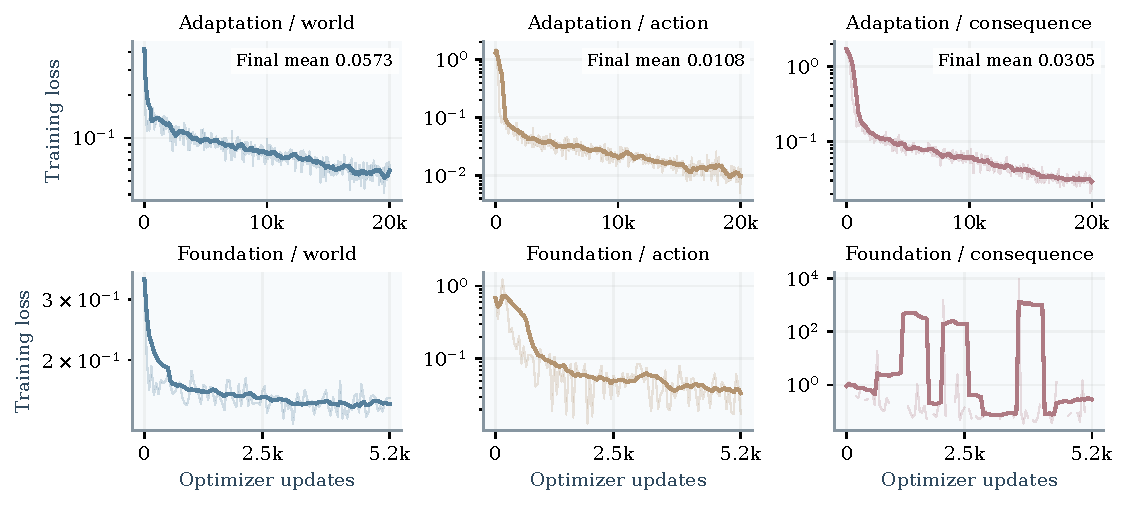
\includegraphics[width=\linewidth]{Figures/training.pdf}
\caption{\textbf{Joint optimization of world, action, and consequence prediction.} Foundation pretraining (top) and completed LIBERO adaptation (bottom). Thin traces retain logged batches; thick traces average up to 11 records with available supervision. Each objective uses a logarithmic scale. Vertical rules mark configuration boundaries, where smoothing restarts. The last foundation segment contains one logged update. Appendix~\ref{app:details} records the changes at each boundary.}
\label{fig:training}
\end{figure}

\FloatBarrier
\subsection{Representation and reciprocal computation}
Figure~\ref{fig:representation} compares motor-action and visual-consequence readout from JAM world features with video and random initialization.
\begin{figure}[!t]
\centering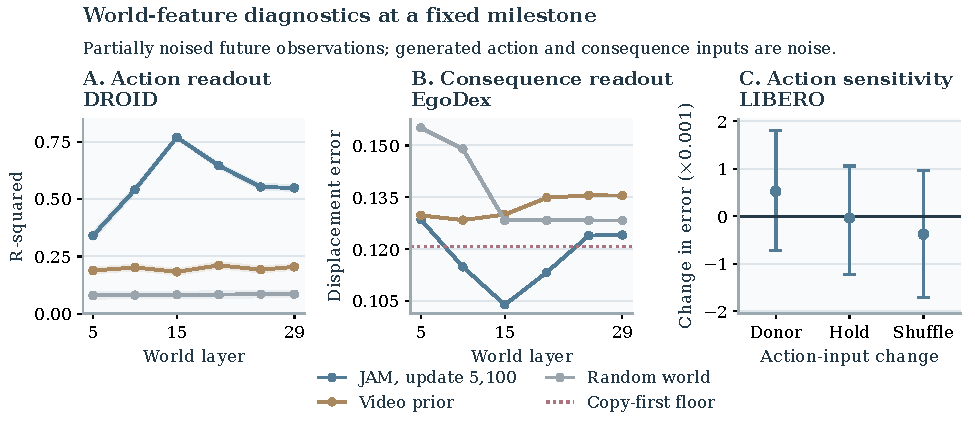
\includegraphics[width=\linewidth]{Figures/representation.pdf}
\caption{\textbf{Reading actions and visual consequences from world features.} Frozen-world ridge probes compare JAM at update 5,100 with video and random initialization at every sampled layer. Top: action R-squared (higher is better) and consequence average displacement error, ADE (lower is better). Bottom: JAM's gain over the video prior, shown as point estimates. The copy-first reference remains visible in B. Action bands use 1,000 window-bootstrap resamples. Future observations are partly visible; the 2,800/1,200 probe-training/test windows can share episodes (Appendix~\ref{app:controls}). Action-input sensitivity is evaluated separately in Figure~\ref{fig:action_sensitivity}, where all paired intervals include zero.}
\label{fig:representation}
\end{figure}

Table~\ref{tab:joint} separates the value of embodied pretraining from the information and gradient paths within joint computation.
% PLANNED-VALUE: superscript T identifies design values awaiting measurement.
\begin{table}[H]
\centering
\begingroup\fontsize{9}{10.5}\selectfont
\setlength{\tabcolsep}{3.5pt}\renewcommand{\arraystretch}{1.12}
\begin{tabularx}{\linewidth}{lRR}
\toprule
\panelrow{3}{A. Initialization at matched adaptation budget}
Initialization & LIBERO & Plus \\
\midrule
Without embodied pretraining & \target{97.2} & \target{53.8} \\
\jamshade\textbf{JAM pretraining} & \target{99.4} & \target{90.2} \\
\bottomrule
\end{tabularx}
\vspace{2pt}
\begin{tabularx}{\linewidth}{lRRRRRRR}
\toprule
\panelrow{8}{B. Information exchange and gradient routing}
Variant & W reads A & A reads W & Gradient & LIBERO & Plus & A probe & C error \\
\midrule
World only & Off & Off & Off & \target{94.0} & \target{42.0} & \target{0.30} & \target{0.18} \\
Action only & Off & Off & Off & \target{95.0} & \target{45.0} & \target{0.32} & \target{0.17} \\
Independent & Off & Off & Off & \target{96.1} & \target{47.6} & \target{0.38} & \target{0.15} \\
Auxiliary & Off & On & Off & \target{96.8} & \target{49.4} & \target{0.40} & \target{0.12} \\
One-way & Off & On & On & \target{97.0} & \target{51.7} & \target{0.46} & \target{0.10} \\
\jamshade{}\textbf{JAM joint} & On & On & On & \target{97.2} & \target{53.8} & \target{0.52} & \target{0.08} \\
\bottomrule
\end{tabularx}
\endgroup
\caption{\textbf{Which part of pretraining changes the representation?} Panel A isolates embodied pretraining from task adaptation. Panel B holds source exposure and clean conditions fixed. W and A denote world and action; Gradient denotes action-loss access to world parameters. A probe reports R-squared; C error is consequence average displacement error (ADE). All entries in this controlled study await measurement. \targetnote}
\label{tab:joint}
\end{table}


\FloatBarrier
\subsection{Data, capacity, and supervision}
Table~\ref{tab:data_scaling} and Figure~\ref{fig:scaling} organize matched-budget comparisons of supervision, unique data, duration, and capacity.
% PENDING-MEASUREMENT: empty result cells await archived experimental evidence.
\begin{table}[H]
\centering
\begingroup\fontsize{9}{10.5}\selectfont
\setlength{\tabcolsep}{3.5pt}\renewcommand{\arraystretch}{1.12}
\begin{tabularx}{\linewidth}{lRRRRRR}
\toprule
\panelrow{7}{A. Which supervision source contributes?}
Mixture & Robot budget & Human & Human C & LIBERO & Plus & C error \\
\midrule
Robot & Matched & Off & Off &  &  &  \\
+ human video & Matched & On & Off &  &  &  \\
\jamshade\textbf{JAM mixture} & Matched & On & On &  &  &  \\
\bottomrule
\end{tabularx}
\vspace{2pt}
\begin{tabularx}{\linewidth}{lRRRR}
\toprule
\panelrow{5}{B. Capacity and supervision density}
Axis & Setting & Corpus & Updates & Plus \\
\midrule
Agent width & 768 & Full & 60k &  \\
\jamshade{}Agent width & 1024 & Full & 60k &  \\
Agent width & 1280 & Full & 60k &  \\
\midrule
Action labels & 25\% & Full & 60k &  \\
Action labels & 50\% & Full & 60k &  \\
\jamshade{}Action labels & 100\% & Full & 60k &  \\
\bottomrule
\end{tabularx}
\endgroup
\caption{\textbf{Which data and scale choices support action grounding?} Panel A matches robot exposure; Panel B fixes the backbone, corpus, and update budget. Success is in percent and C error is image-normalized ADE. Blue rows identify reference settings. \pendingstudynote}
\label{tab:data_scaling}
\end{table}

\begin{figure}[H]
\centering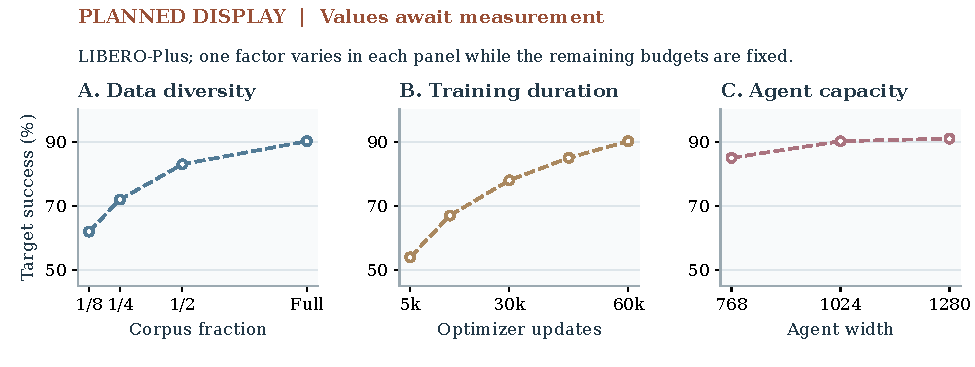
\includegraphics[width=\linewidth]{Figures/scaling_targets.pdf}
\caption{\textbf{How are data and compute effects separated?} Planned LIBERO-Plus displays vary unique data, duration, or agent width at otherwise fixed budgets. All points are PLANNED-VALUE, awaiting measurement; the full-corpus reference uses 60,000 updates.}
\label{fig:scaling}
\end{figure}
\FloatBarrier
